%!TEX root = ../template.tex
%%%%%%%%%%%%%%%%%%%%%%%%%%%%%%%%%%%%%%%%%%%%%%%%%%%%%%%%%%%%%%%%%%%%
%% my-chapter1.tex
%% NOVA thesis document file
%%
%% Chapter with the template manual
%%%%%%%%%%%%%%%%%%%%%%%%%%%%%%%%%%%%%%%%%%%%%%%%%%%%%%%%%%%%%%%%%%%%
%\usepackage{amsmath}
%\usepackage[table]{xcolor}
%\usepackage{xltabular}
%%\usepackage{colortbl} % Added this line
%\usepackage{booktabs}
%\usepackage{enumitem}
%\usepackage{tikz}
%\usetikzlibrary{shapes, arrows, positioning, fit}


\typeout{NT FILE my-chapter2.tex}%

\chapter{Research Statement}
\label{ch:research-statement}

\glsresetall

\section{Introduction}
\label{sec:rs_intro}

    The global energy landscape is undergoing a transformative shift towards sustainability,
    with an increasing reliance on renewable energy sources.
    The integration of wind and solar assets into energy portfolios presents unique challenges,
    necessitating a thorough investigation into effective hedging strategies.
    This thesis research seeks to address these challenges by focusing on the development of robust models and strategies
    for managing wind and solar assets within a realistic portfolio context.

\section{Objectives of the Research}
    \label{sec:rs_objectives}

%\subsection{Problem Definition}
%    \label{subsec:rs_problem-definition}

    The central problem addressed in this research is the effective hedging of renewable energy sources,
    specifically wind and solar, within the complexity of a realistic portfolio.
    My research aims to understand and apply sensible derivative weather instruments to hedge wind and solar assets,
    taking into account a certain risk profile.
    In the following subsections, I will present the objectives of the research and some methodologies that have been
    indentified to achieve them.

\subsection{Forecasting Electricity Spot Prices}
    \label{subsec:rs_forecasting-electricity-spot-prices}

    Approaches to modelling electricity prices can be broadly categorised into two groups.
    On one end of the spectrum are methods that heavily borrow from reduced-form models
    commonly employed in equity or interest rate markets.
    Early studies utilised low-dimensional stochastic processes to depict patterns
    such as mean-reversion and seasonalities.
    To account for distinctive price spikes not observed in other commodity markets,
    various researchers explored variations of jump processes.\\

    The opposite end of the spectrum involves structural production cost models, also known as fundamental models.
    In these modelling approaches, wholesale market clearing prices arise from a cost minimisation problem
    where demand needs to be met while adhering to specific constraints, such as transmission limitations.
    This approach necessitates comprehensive information on the technical specifics of power plants and
    the environmental constraints of the entire power market under consideration.\\

    \textbf{\textit{Methodology: }} Although from work experience, I am familiar with the fundamentals models.
    If applied to the MIBEL market, I am inclined to use the reduced-form models, such as the SMAaPS mode\cite{burger_spot_2004}.

\subsection{Forecasting Wind Speed and Solar Irradiance}
    \label{subsec:rs_forecasting-wind-speed-and-solar-irradiance}

    Predicting wind speed and solar irradiance with precision is imperative for optimising the performance of
    wind and solar assets.
    This research endeavors to develop meteorological models that account for specific asset locations and heights.\\

    \textbf{\textit{Methodology: }} Leveraging advanced meteorological models,
    such as econometrics or multivariate models\cite{benth_multivariate_2019},
    to simulate and predict wind speed and solar irradiance.


\subsection{Computing Load Based on Weather Conditions}
    \label{subsec:forecasting-load-based-on-weather-conditions}

    The interdependence of load on forecasted weather conditions is a critical factor in energy management.
    This research aims to integrate forecasted wind speeds and solar irradiance into independent asset properties,
    e.g. \ power and location, to calculate load forecasting models.\\

\textbf{\textit{Methodology: }} Defining and apply parametric asset properties, such as power and location,
    to compute load forecasting models.

\subsection{Stochastic Interest Rate Structure}
    \label{subsec:rs_stochastic-interest-rate-structure}

    The stochastic nature of interest rates necessitates approach to modelling discounted cash flows would bring a
    more robust analysis and provide essential insights to when would be the best time to perform hedging operation.\\

    \textbf{\textit{Methodology: }} Utilizing stochastic calculus
    and financial modelling techniques\cite{filipovic_term-structure_2009}.

\subsection{Discounted Cash Flow}
    \label{subsec:rs_stochastic-process-for-discounted-cash-flow}

    The uncertainty associated with renewable energy projects requires a
    stochastic approach to model discounted cash flows.
    This research seeks to develop a Monte Carlo analysis of the wind, prices and interest rates stochastic processes.
    This approach will allow to capture these uncertainties and be able to obtain sensible
    distributions of key financial metrics, such as NPV and VAR.\\

    \textbf{\textit{Methodology: }} Monte Carlo Analysis of the wind,
    prices and interest rates stochastic processes, to obtain discounted cash flows.


\subsection{Sensitivity Analysis for Wind/Solar Location}
    \label{subsec:rs_sensitivity-analysis-for-wind/solar-location}

    Understanding the sensitivity of wind speeds and solar irradiation for each asset location
    is essential for understanding individual asset performance and best locations to generate value.\\

    \textbf{\textit{Methodology: }} Conducting sensitivity analyses to assess the impact
        of turbine location on financial outcomes.

\subsection{Literature Review on Weather Derivatives}
    \label{subsec:rs_literature-review-on-weather-derivatives}

    A comprehensive review of existing literature on weather derivatives is essential for understanding their
    applications and limitations in the energy sector.
    Conducting a systematic literature review to synthesize existing knowledge on
    weather derivatives and their applications in the energy sector.

\subsection{Assessment of Derivatives and Their Pricing Models for Hedging}
    \label{subsec:rs_assessment-of-derivatives-and-pricing-models}

    An analysis of existing derivatives and their pricing models is crucial for identifying
    relevant instruments for hedging renewable energy sources.
    The objective is to compile and analyse available weather derivatives products from industry and their
    associated pricing models to assess their applicability to the renewable energy context,
    particularly for wind speeds and solar irradiance.

\subsection{Pricing Options of Weather Derivatives}
    \label{subsec:rs_pricing-options-of-weather-derivatives}

    Understanding the intricacies of pricing weather derivatives, especially in the context of renewable energy,
    would be critical for effective risk management.\\

\textbf{\textit{Methodology: }} Investigating and applying quantitative energy finance methods\cite{benth_quantitative_2014} to price appropriate
    weather derivatives, collated in the previous subsection~\ref{subsec:rs_assessment-of-derivatives-and-pricing-models}.

and option pricing models.
Determine appropriate pricing mechanisms for weather derivatives.

\subsection{Develop Hedging Strategies for Wind/Solar}
    \label{subsec:rs_exploration-of-hedging-strategies-for-wind/solar}

    Developing and evaluating effective hedging strategies tailored to the specific
    characteristics of wind and solar assets is a key focus of this research.\\
    In Figure~\ref{fig:cash-flow-model} is presented a diagram of how these different models would fit.\\

    \textbf{\textit{Methodology: }} Employing quantitative methods, such as option pricing models and risk management
    frameworks, to design and assess hedging strategies for wind and solar assets.

    \begin{figure}
        \centering
        \begin{tikzpicture}[
            rectangle,
            draw,
            node distance=3cm,
            every node/.style={align=center, minimum width=2cm, minimum height=1cm},
            >=stealth
        ]
    %%        % Load library
            \usetikzlibrary{positioning}
            % Nodes
            \node[rectangle, draw, fill=green!30] (spotprices) {Spot Prices};
            \node[rectangle, draw, above=of spotprices, fill=purple!80!blue!20] (wind) {Wind Speed};
            \node[rectangle, draw, right=of wind] (load) {Load};
            \node[rectangle, draw, below=of load] (d_cash_flows) {Discounted Cash Flows};
            \node[rectangle, draw, right=of load] (t_prop) {Asset properties};
            \node[rectangle, draw, right=of d_cash_flows, fill=tz_myblue] (hedging) {Hedging Payoff};
            \node[rectangle, draw, below=1cm of t_prop, above=0.6cm of hedging, fill=tz_myblue] (pricing) {Pricing Options};
            \node[rectangle, draw, below=1cm of wind, above=0.6cm of spotprices, fill=green!30] (i_rate) {Interest Rate};
            % Box
            \node [
                draw,
                fit= (wind),
                inner sep=5pt,
                label={[label distance=-2mm]above:{BSTS}}
            ] {};
            \node [
                draw,
                fit= (i_rate) (spotprices),
                inner sep=5pt,
                label={[label distance=-2mm]above:{Stochastic Processes}}
            ] {};
            \node [
                draw,
                fit= (pricing) (hedging),
                inner sep=5pt,
                label={[label distance=-2mm]above:{Hedging Strategies}}
            ] {};
            \node [
                draw,
                fit= (d_cash_flows),
                inner sep=5pt,
                label={[label distance=-2mm]below:{Monte Carlo}}
            ] {};


            % Arrows
            \draw [->] (spotprices) -- node[midway, above] {} (d_cash_flows);
            \draw [->] (wind) -- node[midway, above] {} (load);
            \draw [->] (t_prop) -- node[midway, above] {} (load);
            \draw [->] (load) -- node[midway, left] {} (d_cash_flows);
            \draw [->] (pricing) -- node[midway, right] {} (hedging);
            \draw [->] (hedging) -- node[midway, above] {} (d_cash_flows);
            \draw [->] (wind) -- node[midway, above] {} (hedging);
            \draw [->] (i_rate) -- node[midway, above] {} (d_cash_flows);
            \draw [->] (i_rate) -- node[midway, above] {} (pricing);

        \end{tikzpicture}
        \caption{Hedged Discounted Cash Flow Models.}
        \label{fig:cash-flow-model}
    \end{figure}

% Please applly same format as above
\subsection{Analysis of Hedging Efficiency}
    \label{subsec:rs_analysis-of-hedging-efficiency}

    Comparing the financial performance of unhedged portfolios against portfolios employing different hedging strategies
    provides insights into their efficiency.
    Also understanding the impact on different technologies, in this case wind and solar and respective asset
    locations.\\

    \textbf{\textit{Methodology: }} Conducting empirical analyses and performance evaluations to assess the
    impact of hedging on financial outcomes.

% Please applly same format as above
\subsection{Risk-Averse Profiles}
    \label{subsec:rs_risk-averse-profiles}

    Exploring various risk-averse profiles and their implications for portfolio optimisation forms
    a critical component of this research.
    Analysing risk preferences through utility functions and exploring how
    different risk-averse profiles influence portfolio strategies.
    Formulating an objective function based on risk aversion is crucial for optimising renewable energy portfolios.\\

    \textbf{\textit{Methodology: }} Utilizing fuzzy logic to map profiles to hedge hyperparameter and use optimisation techniques to define objective
    functions that align with different risk aversion metrics.
    This could be done by defining objective functions such as:
    \begin{enumerate} %[label=\alph*)]
        \item max: Hedged-NPV (Prone to risk)
        \item min: Earning at risk (Risk-averse)
        \item min: Revenue variance (Risk-averse)
    \end{enumerate}
\subsection{Portfolio Optimisation of Wind/Solar}
    \label{subsec:rs_portfolio-optimization-of-wind/solar}

    Examining the integration of wind and solar assets into broader energy portfolios and understanding
    their interactions with non-renewable sources is a key focus of this research.\\

    \textbf{\textit{Methodology: }} Implementing advanced optimisation algorithms, such as linear programming or
    stochastic optimisation, to identify optimal portfolio allocations that maximise returns
    while considering risk factors.

\subsection{Impact of Growing Penetration of Renewable Energy Sources}
    \label{subsec:rs_impact-of-growing-penetration-of-renewable-energy-sources}

    Assessing the market dynamics and economic implications of the increasing renewable penetration in the
    energy generation mix is crucial for understanding the broader context and potential impact of this the research.

%\section{Methodologies}
%    \label{sec:rs_methodologies}
%
%    The proposed research adopts a multidisciplinary approach that combines forecasting, meteorology
%    finance, and optimisation techniques:
%
%    \begin{itemize}
%        \item \textbf{Forecast Models:} Leveraging advanced meteorological models for accurate wind speed and solar
%            irradiance forecasts, considering asset locations and heights.
%        \item \textbf{Financial Modelling:} Employing stochastic models for discounted cash flow, pricing models for
%            weather derivatives, and quantitative methods for hedging strategies and risk management.
%        \item \textbf{Statistical Analysis:} Using statistical and machine learning techniques for
%            forecasting spot prices, loads, and conducting sensitivity analyses.
%        \item \textbf{Literature Review:} Conducting a comprehensive literature review to synthesise existing
%            knowledge on weather derivatives and their applications in the energy sector.
%        \item \textbf{Case Studies:} Integrating real-world case studies to validate and refine forecasting
%            and hedging strategies.
%        \item \textbf{Optimisation Techniques:} Implementing optimisation algorithms to find optimal
%            hedging strategies and portfolio allocations, considering risk aversion metrics.
%    \end{itemize}

\section{Expected Contributions}
    \label{sec:rs_expected-contributions}

    This research aims to make significant contributions to the field:

    \begin{enumerate}%[label=\arabic*.]
        \item Providing actionable insights into the challenges and opportunities of hedging renewable
            energy sources within realistic portfolios using concrete weather derivatives.
        \item Developing advanced forecasting models and effective hedging strategies for wind and solar assets.
        \item Enhancing the understanding of weather derivatives and their applications in the renewable energy sector.
        \item Offering practical guidance for portfolio optimisation in the context of growing
             renewable energy penetration.
    \end{enumerate}

\newpage

\section{Chronogram}
\label{sec:rs_chronogram}

    The following chronogram in Figure~\ref{fig:chronogram}, presents the expected timeline for the completion
    of the research:

    \begin{figure}[htbp]
        \centering
        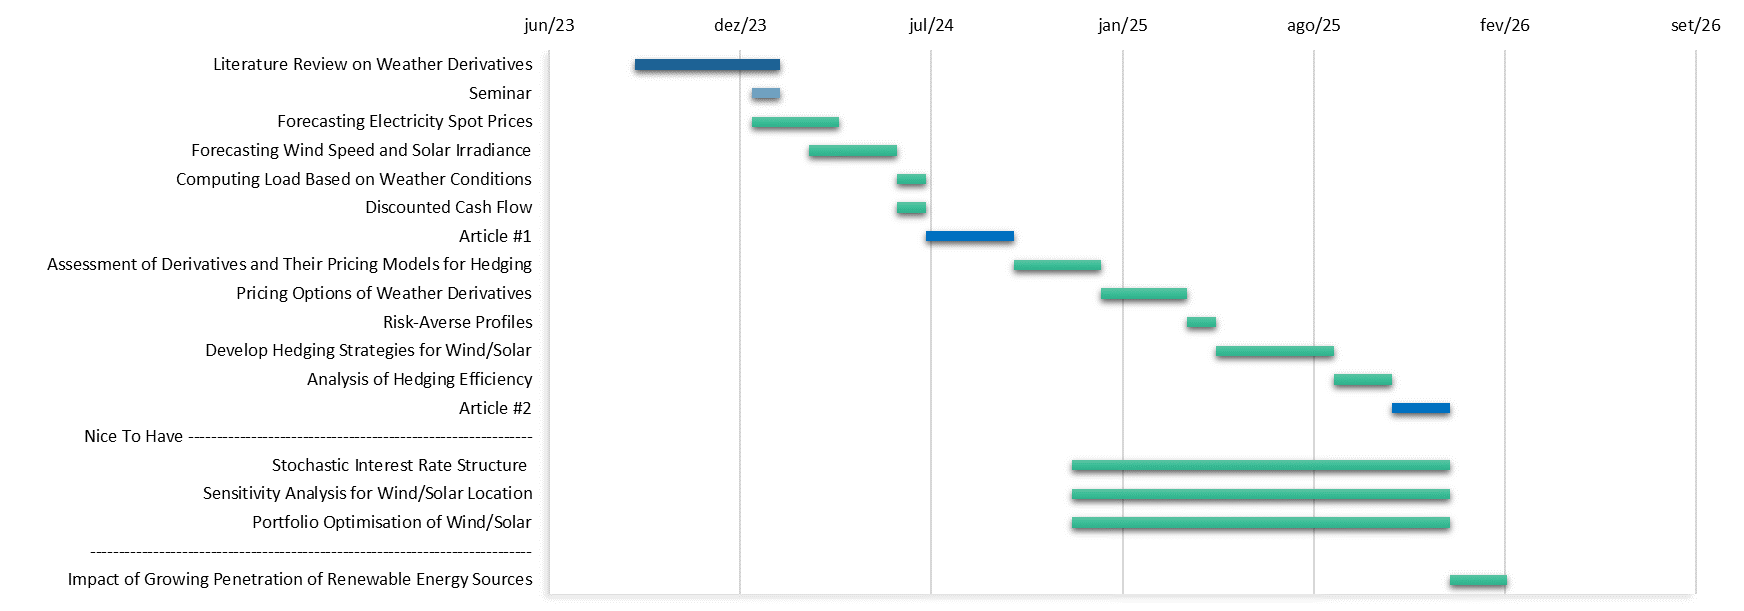
\includegraphics[width=1\textwidth]{Images/CAT/chronogram.png}
        \caption{Research Chronogram.}
        \label{fig:chronogram}
    \end{figure}
%


In conclusion, this Ph.D.\ thesis endeavours to advance knowledge in renewable energy finance and risk management,
offering valuable tools and strategies for stakeholders in the evolving energy landscape.
to support energy management in this challenging path to a secure and sustainable energy transition.




